\documentclass[10pt]{amsart}
% \usepackage[showboxes]{textpos}

\usepackage[absolute,overlay]{textpos}
\setlength{\TPHorizModule}{1.0cm}
\setlength{\TPVertModule}{\TPHorizModule}
\textblockorigin{0.0cm}{0.0cm}  %start all at upper left corner

\usepackage{lmodern}
\usepackage{amsmath}
\usepackage{amsthm}
\usepackage{amsfonts}
\usepackage{amssymb}
\usepackage{mathpazo}
\usepackage{booktabs}
\usepackage[usenames,x11names]{xcolor}
\usepackage{tikz}
\usepackage{textcomp}
\usepackage[letterpaper]{geometry}
\geometry{verbose,tmargin=0.5in,bmargin=0.5in,lmargin=0.75in,rmargin=0.5in}
\usepackage{multicol}
\usepackage{bm}
\usepackage{comment}
\usepackage{cancel}
\usepackage{array}
\usepackage{gensymb}
\usepackage{enumerate}

\pagestyle{plain}
\raggedright
\renewcommand{\familydefault}{\sfdefault}
\setlength{\parskip}{\medskipamount}
\setlength{\columnsep}{1cm}

\everymath{\displaystyle}
\setlength{\parskip}{\bigskipamount}

% counter for resuming enumerated list numbers
\newcounter{resumeenumi}
\newcommand{\suspend}{\setcounter{resumeenumi}{\theenumi}}
\newcommand{\resume}{\setcounter{enumi}{\theresumeenumi}}

\newcommand\lb{\linebreak}
\newcommand\pars{\par\smallskip}
\newcommand\parm{\par\medskip}
\newcommand\parb{\par\bigskip}

\makeatletter
\providecommand{\gettikzxy}[3]{%
	\tikz@scan@one@point\pgfutil@firstofone#1\relax
	\edef#2{\the\pgf@x}%
	\edef#3{\the\pgf@y}%
}
\makeatother



% full width colored block but color specifiable
%\cb[body bg strength]{header bg}{header text}{body text}
\newcommand{\cb}[4][15]{
	\setbeamercolor{block title}{bg = #2}
	\setbeamercolor{block body}{bg = #2!#1}
	\setbeamercolor{item projected}{bg=#2, fg=white}
	\begin{center}
		\begin{block}{#3}
			#4
		\end{block}
	\end{center}
}

% colored block with width specified
% \cbw[body bg strength]{header bg}{width}{header text}{body text}
\newcommand{\cbw}[5][15]{
	\begin{center}
		%\vspace{-0.35cm}
		\begin{minipage}{#3\textwidth}
			\setbeamercolor{block title}{bg= #2}
			\setbeamercolor{block body}{bg= #2!#1}
			\setbeamercolor{item projected}{bg=#2, fg=white}
			\begin{block}{#4}
				\raggedright
				#5
			\end{block}
		\end{minipage}
	\end{center}
}

% centered minipage with text \raggedright
%\cmini[width]{content}
\newcommand{\cmini}[2][0.8]{
	\begin{center}
		\begin{minipage}{#1\columnwidth}
			\raggedright
			#2
		\end{minipage}
	\end{center}
}

%left flushed minipage
\newcommand{\mini}[2][0.8]{
	\begin{minipage}{#1\columnwidth}
		\raggedright
		#2
	\end{minipage}
}

%left flushed minipage, top aligned
\newcommand{\minit}[2][0.8]{
	\begin{minipage}[t]{#1\columnwidth}
		\raggedright
		#2
	\end{minipage}
}

%left flushed minipage
% \newcommand{\miniT}[2][0.8]{
%  \begin{minipage}[T]{#1\columnwidth}
%   \raggedright
%   #2
%  \end{minipage}
% }

%left flushed minipage
\newcommand{\minib}[2][0.8]{
	\begin{minipage}[b]{#1\columnwidth}
		\raggedright
		#2
	\end{minipage}
}

\newcommand{\cfig}[2][1]{% centred, scaled graphic
	\begin{center}
		\includegraphics[scale=#1]{#2}
	\end{center}
}
% figure with tight border for photos
% \cfigb[saitMaroon]{borderwidth with unit}{scale}{image}
\newcommand{\cfigb}[4][structure]{
	% \usepackage{adjustbox}
	\setlength{\fboxrule}{1pt}
	\begin{center}
		\includegraphics[scale=#3, cframe= #1 #2]{#4}
	\end{center}
}

\newcommand{\imgbox}[3]{
	% \setlength{\fboxsep}{12pt}
	\includegraphics[scale=#1, cframe= structure #3]{#2}
}

% \imgboxbg[bg color=white]{scale}{path/to/img}{border color}{border, e.g. 2pt}{margin, e.g. 4pt}
\newcommand{\imgboxbg}[6][white]{
	\setlength{\fboxrule}{#5}
	\setlength{\fboxsep}{#6}
	\centering
	\fcolorbox{#4}{#1}{\includegraphics[scale=#2]{#3}}
}

\newcommand{\fig}[2][1]{% scaled graphic
	\includegraphics[scale=#1]{#2}
}

% centred framed  box black border
%\cbox[width]{content}
\newcommand{\cbox}[2][0.9]{% framed centered  box
	\setlength\fboxsep{0.042\columnwidth}
	\setlength\fboxrule{0.0015\columnwidth}
	\begin{center}
		\fcolorbox{black}{white}{
			\vspace{-0.5cm}
			\begin{minipage}{#1\columnwidth}
				\raggedright
				#2
			\end{minipage}
		}
	\end{center}
	\setlength\fboxsep{0cm}
}



\newtcolorbox{mybox}[1][]
{
	colback=white,
	top=0.25cm,
	bottom=0.25cm,
	left=0.25cm,
	right=0.25cm,
	colframe=structure,
	fonttitle=\bfseries,
	enhanced, drop fuzzy shadow,
	% attach boxed title to top left={yshift=-2mm, xshift=5mm},
	attach boxed title to top left={yshift=-2mm, xshift=5mm}, colbacktitle=structure!80!white, #1}

\newtcolorbox{plainbox}[1][]{colback=white, sharp corners, top=0.125cm, bottom=0.125cm, left=0pt, right=0pt, boxrule=0.5pt,colframe=structure,fonttitle=\bfseries, colbacktitle=structure, arc=0mm, #1}
%
\newtcbtheorem{myexam}{Example}%
{
	enhanced,
	colback=white,
	top=0.375cm,
	bottom=0.25cm,
	left=0.375cm,
	right=0.375cm,
	colframe=structure,
	fonttitle=\bfseries,
	drop fuzzy shadow,
	%description font=\mdseries\itshape,
	attach boxed title to top left={yshift=-2mm, xshift=5mm},
	colbacktitle=structure!80!white
	}{exam}% then \pageref{exer:theoexample} references the theo

\newcommand{\myexample}[2][red]{
	% \tcb\tcbset{theostyle/.style={colframe=red,colbacktitle=yellow}}
	\begin{myexam}{}{}
		\raggedright
		#2
	\end{myexam}
	% \tcbset{colframe=structure,colbacktitle=structure}
}

\newtcbtheorem{myexer}{Exercise}%
{
	enhanced,
	colback=white,
	top=0.375cm,
	bottom=0.25cm,
	left=0.375cm,
	right=0.375cm,
	colframe=structure,
	fonttitle=\bfseries,
	drop fuzzy shadow,
	%description font=\mdseries\itshape,
	attach boxed title to top left={yshift=-2mm, xshift=5mm},
	colbacktitle=structure!80!white
	}{exer}

\newcommand{\myexercise}[2][red]{
	% \tcb\tcbset{theostyle/.style={colframe=red,colbacktitle=yellow}}
	\begin{myexer}{}{}
		\raggedright
		#2
	\end{myexer}
	% \tcbset{colframe=structure,colbacktitle=structure}
}


\begin{document}

\thispagestyle{empty}
\vspace{-7cm}
\centering

\textbf{\Large Module 7: Series A Pipeline (CIVL 318)}
\par\medskip


%%%%%%%%%%%%%%%%%%%%%%%%%%%%%%%%%%%%%%%%%%%%%%%%%%%%%%%%%%%%%%%%%%%%%%%%%%%%%%%%%%%%%%%%%%%%%%%%%%%%%%%%%%%%%%%%%%%%%

%\rule{\textwidth}{0.02in}
%%%%%%%%%%%%%%%%%%%%%%%%%%%%%%%%%%%%%%%%%%%%%%%%%%%%%%%%%%%%%%%%%%%%%%%%%%%%%%%%%%%%%%%%%%%%%%%%%%%%%%%%%%%%%%%%%%%%%
\raggedright

\begin{multicols}{2}
	
	
	%%%%%%%%%%%%%%%%%%%%%%%%%%%%%%%%%%%%%%%%%%%%%%%%%%%%%%%%%%%%%%%%%%%%%%%%%%%%%%%%%%%%%%%%%%%%%%%%%%%%%%%%%
	
	
	\textbf{Example 1}:
	
	
	A pump delivers 13.5 L/s of kerosene at $25^\circ$C from an underground vented
	storage tank to an elevated storage tank pressurized to 745 kPa.
	\par
	The suction pipe is 6-in Schedule 40 steel pipe and is $5.0\,\text{m}$ long. It has a round-edged entrance with a radius
	of $r=15$ mm.
	\par
	The discharge pipe is 3-in Schedule 40 steel pipe,  is $11.0\,\text{m}$ long and includes a fully open butterfly valve
	with $L_e/D=45$.
	\par
	All elbows are ``standard'' with $L_e/D=30$.
	
	\cfig[0.4]{../../Figs/07SeriesPipeline/ElevStorA}
	
	\textbf{Solution}:\parb
	\Large
	
	\mini{
		\underline{Suction Pipe}
		
		\cbox[0.9]{
			\begin{align*}
				v              & = \frac{0.0135\,\mathsf{m^3/s}}{\pi(0.1540\,\text{m})^2/4} = 0.72383\,\text{m/s} \\
				\frac{v^2}{2g} & = 0.026704\,\text{m}                                                             \\
				N_R            & = \frac{0.72383(0.1541)823}{1.64\times 10^{-3}} = 55975 \approx 5.6 \times 10^4  \\
			\end{align*}
		}
	}
	
	\vfill\columnbreak
	
	Friction Losses:\\
	\cbox[0.9]{
		\begin{align*}
			\frac{D}{\epsilon} & = \frac{0.1541}{4.6\times 10^{-5}}=3350         \\
			f                  & = 0.0215\quad\text{(Moody)}                     \\
			                   & = 0.02144\quad\text{(Swamee-Jain)}              \\\\
			h_L                & = 0.0215\left(\frac{5.0}{0.1541}\right)0.026704 \\
			                   & = \bm{0.018629\,\text{m}}                       
		\end{align*}
	}
	
	Minor Losses:\\
	\cbox[0.9]{
		\begin{align*}
			f_T                  & = 0.015\quad\text{(Moody)}                                          \\
			K_{\text{entrance}}  & = 0.09\quad\text{($r/D=0.1$)}                                       \\
			K_{\text{elbow}}     & = f_T\left(\frac{L_e}{D}\right) = 0.015(30) = 0.45                  \\
			h_{L_{\text{minor}}} & = K_{\text{entrance}}\frac{v^2}{2g}+2K_{\text{elbow}}\frac{v^2}{2g} \\
			                     & = (0.09+2\times0.45)0.026704                                        \\
			                     & = \bm{0.026437\,\text{m}}                                           
		\end{align*}
	}
	
	\underline{Discharge Pipe}
	
	\cbox[0.9]{
		\begin{align*}
			v              & = \frac{0.0135\,\mathsf{m^3/s}}{\pi(0.0779\,\text{m})^2/4} = 2.8325\,\text{m/s} \\
			\frac{v^2}{2g} & = 0.40892\,\text{m}                                                             \\
			N_R            & = \frac{2.8325(0.0779)823}{1.64\times 10^{-3}} = 110730 \approx 1.1 \times 10^5 \\
		\end{align*}
	}
	
	Friction Losses:\\
	\cbox[0.9]{
		\begin{align*}
			\frac{D}{\epsilon} & = \frac{0.0779}{4.6\times 10^{-5}}=1693         \\
			f                  & = 0.0205\quad\text{(Moody)}                     \\\\
			h_L                & = 0.0205\left(\frac{11.0}{0.0779}\right)0.40892 \\
			                   & = \bm{1.1837\,\text{m}}                         
		\end{align*}
	}
	
	\vfill\pagebreak
	
	Minor Losses:\parm
	\mini{
		\cbox[0.9]{
			\begin{align*}
				f_T                  & = 0.018\quad\text{(Table)}                         \\
				K_{\text{elbow}}     & = f_T\left(\frac{L_e}{D}\right) = 0.018(30) = 0.54 \\
				K_{\text{valve}}     & = f_T\left(\frac{L_e}{D}\right) = 0.018(45) = 0.81 \\
				K_{\text{exit}}      & = 1                                                \\
				h_{L_{\text{minor}}} & = \left(0.54+0.81+1\right)0.40892                  \\
				                     & = \bm{0.96096\,\text{m}}                           
			\end{align*}
		}
		\parm
		Total head losses:\parm
		\cbox[0.9]{
			\begin{align*}
				h_L & = 0.018629 + 0.026437   \\
				    & \quad +1.1837+0.96096   \\
				    & = \bm{2.1897\,\text{m}} 
			\end{align*}
		}
		\parm
		General Energy Equation:\parm
		\cbox[0.9]{
			\begin{align*}
				\cancel{\frac{P_A}{\gamma}} + \cancel{z_A} + \cancel{\frac{v_A^2}{2g}} +h_A-h_L & = \frac{P_A}{\gamma} + z_A +                
				\cancel{\frac{v_A^2}{2g}} \\
				h_A-2.1897                                                                      & = \frac{745}{0.823\times 9.81} + 11.8       \\
				h_A                                                                             & = 106.27\,\text{m}                          \\\\
				P_{\text{added}}                                                                & = h_A \gamma Q                              \\
				                                                                                & = 106.27\left(0.823\times 9.81\right)0.0135 \\
				                                                                                & = 11.583                                    \\\\
				P_I                                                                             & = \frac{11.583}{0.73}                       \\
				                                                                                & = \bm{15.87\,\text{kW}}                     
			\end{align*}
		}
	}
	
	\vfill
	\pagebreak
	
	
	%%%%%%%%%%%%%%%%%%%%%%%%%%%%%%%%%%%%%%%%%%%%%%%%%%%%%%%%%%%%%%%%%%%%%%%%%%%%%%%%%%%%%%%%%%%%%%%%%%%%%%%%%
	
\end{multicols}
\textbf{Example 2}:

Gasoline at $25\text{ \textcelsius}$ flows under gravity from tank $A$ to tank $B$; both tanks are open to the
atmosphere.

The $2$-in Schedule $40$ steel pipe has a square entrance is $45.7\text{	m}$ long. The $4$-in Schedule $40$ steel
pipe contains a fully-open globe valve and is $87.5\text{ m}$ long. There is a sudden enlargement between the two
pipes, as shown. Both pipes are new commercial steel. All elbows are standard $90\degree$.

Determine the difference in surface elevation between tanks $A$
and $B$ required to maintain a flow of $425\text{ L/min}$.

\cfig[0.5]{../../Figs/07SeriesPipeline/07SeriesFindY}

\begin{multicols}{2}
	
	
	\mini{
		\underline{2-in Pipe}
		\parb
		\cbox[0.9]{
			\Large
			\begin{align*}
				v              & = \frac{0.425/60\,\mathsf{m^3/s}}{\pi(0.0525\,\text{m})^2/4} = 3.2721\,\text{m/s} \\
				\frac{v^2}{2g} & = 0.54571\,\text{m}                                                               \\
				N_R            & = \frac{3.2721(0.0525)680}{2.87\times 10^{-4}}                                    \\
				               & = 407020 = 4.07 \times 10^5                                                       \\
			\end{align*}
			$N_R>4000$ so flow is turbulent.
		}
		\parb
		Friction Losses:
		\parb
		\cbox[0.9]{
			\Large
			\begin{align*}
				\frac{D}{\epsilon} & = \frac{0.0525}{4.6\times 10^{-5}}=1141.3      \\
				f                  & = 0.0203\quad\text{(Moody)}                    \\
				                   & = 0.019945\quad\text{(Swamee-Jain)}            \\
				\intertext{Using $f=0.0203$}
				h_L                & = 0.019\left(\frac{45.7}{0.0525}\right)0.54571 \\
				                   & = \bm{9.6431\,\text{m}}                        
			\end{align*}
		}
	}
	
	\vfill\columnbreak
	
	Minor Losses:
	\cbox[0.9]{
		\Large
		\begin{align*}
			f_T                      & = 0.0192\quad\text{(Moody)}                    \\
			                         & = 0.019026\quad\text{(Swamee-Jain)}            \\
			                         & = 0.019\quad\text{(from table for steel pipe)} \\
			\intertext{Use $f=0.019$}
			K_{\text{entrance}}      & = 0.5                                          \\
			2\times K_{\text{elbow}} & = 2\times f_T\left(\frac{L_e}{D}\right)        \\
			                         & = 2\times 0.019(30) = 1.14                     \\
			K_{\text{enlargement}}   & = 0.52                                         \\\\
			\Sigma K                 & = 2.16                                         \\\
			h_{L_{\text{minor}}}     & = \Sigma K\times\frac{v^2}{2g}                 \\
			                         & = (2.16)0.54571                                \\
			                         & = \bm{1.1787\,\text{m}}                        
		\end{align*}
	}
	\vfill\pagebreak
	
	\mini{
		\underline{4-in Pipe}
		
		\cbox[0.9]{
			\Large
			\begin{align*}
				v              & = \frac{0.425/60\,\mathsf{m^3/s}}{\pi(0.1023\,\text{m})^2/4} = 0.86178\,\text{m/s} \\
				\frac{v^2}{2g} & = 0.037852\,\text{m}                                                               \\
				N_R            & = \frac{0.86178(0.1023)680}{2.87\times 10^{-4}}                                    \\
				               & = 208880 = 2.08 \times 10^5                                                        \\
			\end{align*}
			$N_R>4000$ so flow is turbulent.
		}
		\parb
		Friction Losses:
		\parb
		\cbox[0.9]{
			\Large
			\begin{align*}
				\frac{D}{\epsilon} & = \frac{0.1023}{4.6\times 10^{-5}}=2223.9        \\
				f                  & = 0.0177\quad\text{(Moody)}                      \\
				                   & = 0.017661\quad\text{(Swamee-Jain)}              \\
				\intertext{Using $f=0.0177$}
				h_L                & = 0.0177\left(\frac{87.5}{0.1023}\right)0.037852 \\
				                   & = \bm{0.57305\,\text{m}}                         
			\end{align*}
		}
	}
	
	\vfill\columnbreak
	
	Minor Losses:
	\cbox[0.9]{
		\Large
		\begin{align*}
			f_T                      & = 0.0162\quad\text{(Moody)}                    \\
			                         & = 0.016319\quad\text{(Swamee-Jain)}            \\
			                         & = 0.017\quad\text{(from table for steel pipe)} \\
			\intertext{Use $f_T=0.017$}
			K_{\text{exit}}          & = 1                                            \\
			2\times K_{\text{elbow}} & = 2\times f_T\left(\frac{L_e}{D}\right)        \\
			                         & = 2\times 0.017(30) = 1.02                     \\
			K_{\text{globe}}         & = f_T\left(\frac{L_e}{D}\right)                \\
			                         & = 0.017(340) = 5.78                            \\
			\Sigma K                 & = 7.8                                          \\\
			h_{L_{\text{minor}}}     & = \Sigma K\times\frac{v^2}{2g}                 \\
			                         & = (7.8)0.037852                                \\
			                         & = \bm{0.29525\,\text{m}}                       
		\end{align*}
	}
	Total losses in system:
	\cbox[0.9]{
		\Large
		\begin{align*}
			h_L & = 9.6431+1.1787        \\
			    & \quad +0.57305+0.29525 \\
			    & =11.690\,\text{m}      
		\end{align*}
	}
	
	Find $y$
	\cbox[0.9]{
		\Large
		\begin{align*}
			\frac{P_1}{\gamma} +z_1+\frac{v_1^2}{2g}-h_L & = \frac{P_2}{\gamma} +z_2+\frac{v_2^2}{2g} \\
			0+y+0-11.690                                 & = 0+0+0                                    \\
			y                                            & =11.690\,\text{m}                          
		\end{align*}
	}
	
	
	\vfill
	\pagebreak
	
\end{multicols}

%%%%%%%%%%%%%%%%%%%%%%%%%%%%%%%%%%%%%%%%%%%%%%%%%%%%%%%%%%%%%%%%%%%%%%%%%%%%%%%%%%%%%%%%%%%%%%%%%%%%%%%%%


\textbf{Example 3}:

Water at $25\text{ \textcelsius}$ is pumped from tank $A$ to tank $B$.
Both tanks are open to the atmosphere.

The suction pipe is $4\text{-in}$ Schedule $40$ steel pipe, has a well-rounded ($r/D>0.15$) entrance, contains a fully
open globe valve, and is $17.0\text{ m}$ long. The discharge pipe is $3\text{-in}$ Schedule $40$ steel pipe, contains a fully open globe valve and
three standard $90\degree$ elbows; it is $163.3\text{ m}$ long.

The elevation difference between $A$ and $B$ is $12.75\text{ m}$ and the volume flow rate is $Q=900\text{ L/min}$.

If the pump is $78\%$ efficient, determine the electrical power it uses.

\cfig[0.5]{../../Figs/07SeriesPipeline/07SeriesPump}

\begin{multicols}{2}
	
	\textbf{Solution}:\\
	\Large
	\mini{
		\parb
		\underline{\bf Suction Pipe}
		\cbox[0.9]{
			\begin{align*}
				v                    & = \frac{0.900/60\,\mathsf{m^3/s}}{\pi(0.1023\,\text{m})^2/4} = 1.8249\,\text{m/s} \\
				\frac{v^2}{2g}       & = 0.16974\,\text{m}                                                               \\
				N_R                  & = \frac{1.8249(0.1023)997}{8.91\times 10^{-4}} = 208900                           \\
				                     & \approx 2.1 \times 10^5                                                           \\\\
				\frac{D}{\epsilon}   & = \frac{0.1023}{4.6\times 10^{-5}}	= 2223.9                                       \\\\
				f_{\normalsize(S-J)} & = 0.018587                                                                        
			\end{align*}
		}
		
		\parb
		\underline{Head-loss (Friction)}
		\parb
		\cbox[0.9]{
			\begin{align*}
				h_L & = f\frac{L}{D} \frac{v^2}{2g}                     \\
				    & = 0.018587\left( \frac{17}{0.1023}\right) 0.16974 \\
				    & = 0.52432\text{ m}                                
			\end{align*}
		}
	}
	
	\vfill
	\columnbreak
	
	\mini{
		
		\parb
		\underline{Head-loss (Minor)}
		\parb
		\cbox[0.9]{
			\begin{align*}
				f_T       & = 0.017                                \\
				k_{ent}   & = 0.04                                 \\
				k_{valve} & = 0.017(340)	= 5.78                    \\\\
				h_L       & = \left(\Sigma k \right)\frac{v^2}{2g} \\
				          & = 5.82(0.16975)                        \\
				          & = 0.98795\text{ m}                     
			\end{align*}
		}
	}
	
	\underline{\bf Discharge Pipe}
	
	\cbox[0.9]{
		\begin{align*}
			v                    & = \frac{0.900/60\,\mathsf{m^3/s}}{\pi(0.0779\,\text{m})^2/4} = 3.1472\,\text{m/s} \\
			\frac{v^2}{2g}       & = 0.50484\,\text{m}                                                               \\
			N_R                  & = \frac{3.1472(0.0779)997}{8.91\times 10^{-4}} = 274330                           \\
			                     & \approx 2.74 \times 10^5                                                          \\
			\frac{D}{\epsilon}   & = \frac{0.0779}{4.6\times 10^{-5}}	= 1693.5                                       \\
			f_{\normalsize(S-J)} & = 0.018941                                                                        
		\end{align*}
	}
	
	\vfill
	\pagebreak
	
	\parb
	\underline{Head-loss (Friction)}
	\parb
	\mini{
		
		\cbox[0.9]{
			\begin{align*}
				h_L & = f\frac{L}{D} \frac{v^2}{2g}                        \\
				    & = 0.018941\left( \frac{163.3}{0.0779}\right) 0.50484 \\
				    & = 20.045\text{ m}                                    
			\end{align*}
		}
		
		\parb
		\underline{Head-loss (Minor)}
		\parb
		\cbox[0.9]{
			\begin{align*}
				f_T        & = 0.018                                \\
				k_{exit}   & = 1                                    \\
				k_{elbows} & = 3\times 0.018(30)                    \\
				           & = 1.62                                 \\
				k_{valve}  & = 0.018(340)	= 6.12                    \\\\
				h_L        & = \left(\Sigma k \right)\frac{v^2}{2g} \\
				           & = 8.74(0.50484)                        \\
				           & = 4.4123\text{ m}                      
			\end{align*}
		}
		
		\parb
		\underline{Total Head-loss}
		\parb
		\cbox[0.9]{
			\begin{align*}
				      & 0.52432            \\
				      & 0.98795            \\
				      & 20.045             \\
				      & \underline{4.4123} \\
				h_L	= & 25.970             
			\end{align*}
		}
		
	}
	
	\vfill
	\columnbreak
	
	\parb
	\underline{General Energy Equation}
	\parb
	\cbox[0.9]{
		\begin{align*}
			\frac{P_1}{\gamma} +z_1+\frac{v_1^2}{2g}+h_A -h_L & = \frac{P_2}{\gamma} +z_2+\frac{v_2^2}{2g} \\
			0+0+0+h_A-25.970                                  & = 0+12.75+0                                \\
			h_A                                               & =38.720\,\text{m}                          \\
			pow_{added}                                       & = h_A \gamma Q                             \\
			                                                  & = 38.720 (9.78) (0.900/60)                 \\
			                                                  & = 5.6802\text{ kW}                         \\\\
			pow_{drawn}                                       & = \frac{pow_{added}}{e_M}                  \\
			                                                  & = \frac{5.6802}{.78}                       \\
			                                                  & = 7.28\text{ kW}                           
		\end{align*}
	}
	
	\vfill
	
	
	
	
	
	\pagebreak
\end{multicols}

%%%%%%%%%%%%%%%%%%%%%%%%%%%%%%%%%%%%%%%%%%%%%%%%%%%%%%%%%%%%%%%%%%%%%%%%%%%%%%%%%%%%%%%%%%%%%%%%%%%%%%%%%

\textbf{Example 4}:

\begin{multicols}{2}
	Heavy machine oil (sg=$0.89$ and $\eta=3.80\times10^{-2}\mathsf{\ Pa\cdot s}$) is circulated through a system repeatedly to test its stability. \par\medskip
	The 8-inch Schedule steel pipe on the suction side of the pump has a square entrance and a length of $6.25$ m and the
	3.5-inch Schedule steel pipe on the discharge side of the pump has a length of $18.0$ m. All elbows are long
	radius. The flow rate through the system is $13.5$ L/s. \par\medskip
	Determine the head added by the pump. \par\medskip
	\columnbreak
	\cfig[0.35]{../../Figs/07SeriesPipeline/07SeriesCycleOil}
	
\end{multicols}

\begin{multicols}{2}
	
	\textbf{Suction Pipe}:\parm
	
	\cbox[0.9]{
		\begin{align*}
			v              & = \frac{0.0135\ \mathsf{m^3/s}}{\pi(0.2027)^2/4}=0.41835 \text{ m/s} \\
			\frac{v^2}{2g} & = 0.0089202\,\text{m}                                                \\
			N_R            & = \frac{0.41835(0.2027)890}{3.80\times10^{-2}}                       \\
			               & = 1986.1                                                             
		\end{align*}
	}
	
	Flow is laminar.
	
	\cbox[0.9]{
		Friction losses:\\
		\begin{align*}
			f   & = \frac{64}{N_R}\ =\ \frac{64}{1986.1}\ =\ 0.032224          \\
			h_L & = 0.032224\left(\frac{6.25}{0.2027}\right)0.0089202\text{ m} \\
			    & =0.0088630\text{ m}                                          
		\end{align*}
	}
	
	
	\cbox[0.9]{
		Minor Losses:\\
		\begin{align*}
			k_{ent} & = 0.5                          \\
			h_L     & = 0.5\times 0.0089202\text{ m} \\
			        & =0.0044601\text{ m}            
		\end{align*}
	}
	
	\vfill\columnbreak
	
	\textbf{Discharge Pipe}:\par\medskip
	
	\cbox[0.9]{
		\begin{align*}
			v              & = \frac{0.0135\ \mathsf{m^3/s}}{\pi(0.0901)^2/4}=2.1174 \text{ m/s} \\
			\frac{v^2}{2g} & = 0.22850\,\text{m}                                                 \\
			N_R            & = \frac{2.1174(0.0901)890)}{3.80\times10^{-2}}=4468.2               
		\end{align*}
	}
	
	Flow is turbulent.
	
	\cbox[0.9]{
		Friction losses:\\
		\begin{align*}
			\frac{D}{\epsilon} & = \frac{0.0901}{4.6\times 10^{-5}}                      \\\\
			f                  & \quad 0.039\,\text{(Moody)}                             \\
			                   & = \text{(}0.039792\,\text{from S-J)}                    \\
			h_L                & = 0.039\left(\frac{18.0}{0.0901}\right)0.22850\text{ m} \\
			                   & =1.7803\text{ m}                                        
		\end{align*}
	}
	
	\cbox[0.9]{
		Minor losses:
		\begin{align*}
			f_T             & = 0.0165\,\text{Moody}                  \\
			3\times k_{elb} & = 3(0.0165)(20) = 0.99                  \\
			h_L             & = 0.99\times 0.22850 = 0.22622\text{ m} 
		\end{align*}
	}
	
\end{multicols}

\pagebreak

\cmini{
	Total headloss = $ 2.0198$ m\parb
	
	Head added by the pump is found by applying the GEE to the surface of the tank ($A$) and the outlet from the discharge pipe ($B$):
	
	\begin{align*}
		\cancelto{0}{\frac{P_A}{\gamma}}+\cancelto{0}{z_A}+\cancelto{0}{\frac{v_A^2}{2g}}+h_A-h_L & = \cancelto{0}{\frac{P_B}{\gamma}}+z_B+\frac{v_B^2}{2g} \\
		h_A-2.0198                                                                                & = 0.425+0.22850                                         \\\\
		h_A                                                                                       & \approx 2.67\text{ m}                                   \\
	\end{align*}
}

\vfill
\pagebreak


%%%%%%%%%%%%%%%%%%%%%%%%%%%%%%%%%%%%%%%%%%%%%%%%%%%%%%%%%%%%%%%%%%%%%%%%%%%%%%%%%%%%%%%%%%%%%%%%%%%%%%%%%

\textbf{Example 5}:




The system illustrated is a pumped storage system. During periods of high demand for electricity, water flows down
from the upper lake and drives the turbine at $D$. (During periods of low demand when electricity is cheap, such as at
night-time, $D$ acts as a pump and pumps water back up to the upper lake.)
\par\medskip
At times of maximum demand, the system has a maximum volume flow rate of $420\;\mathsf{m^3/s}$. Base your
calculations on this flow. The water is at $10\text{\textcelsius}$.
\par\medskip
The difference in elevation between the surfaces of the two lakes is $542\text{	m}$. \par\medskip
The low pressure tunnel from $A$ to $B$ is $1700\text{ m}$ in length, has a diameter of $10.5\text{ m}$
and is lined with concrete. The shaft and high pressure tunnel from $B$ to $D$ is $1140\text{ m}$ in length, has a diameter of $10.5\text{ m}$ and
is lined with welded steel.
\par\medskip
There are three tailrace tunnels from the turbine to the lower reservoir with the flow equally
distributed between them. Each tailrace tunnel is $382\text{ m}$ in
length, has a diameter of $8.5\text{ m}$ and is lined with concrete.

\par\medskip
The entrance to the low pressure tunnel at the upper lake has an equivalent length ratio of $Le/D=420$. The bends at
$B$ and $C$ are in the steel pipe and each have at equivalent length ratio of $16$. A spherical valve at the
inlet of the turbine that shuts off flow when the turbines are not operating is hydraulically efficient and has no
losses associated with it. Each tailrace tunnel contains a butterfly valve ($Le/D=20$).
\par\medskip
At maximum capacity, the turbine outputs $1800 \text{ MW}$. Determine the efficiency of the turbine at this output.

\cfig[0.5]{../../Figs/07SeriesPipeline/series2}
\textbf{Solution}:\\

% (Text in \textcolor{red}{red} is	explanatory and is not required in your solution.)
%
% \textcolor{red}{Series pipelines problems require finding the head losses, both due to friction and minor
% losses, to find the total head loss in the system. Then the General Energy Equation is applied, using the combined head losses already
% calculated.}

\textbf{Pipe AB}

\textcolor{blue}{\em Velocity and velocity head in the $10.5$ m diameter tunnel}:\\

\begin{gather*}
	v = \frac{Q}{A} = \frac{420\mathsf{\;m^3/s}}{\pi(10.5\mathsf{ m})^2/4}=4.8504\mathsf{\ m/s} \\\\
	\frac{v^2}{2g} = \frac{(4.8504\mathsf{\;m/s})^2}{2\times9.81\mathsf{\;m/s^2}} = 1.1991\mathsf{\; m}
\end{gather*}

\textcolor{blue}{\em Reynolds Number, relative roughness and friction factors for tunnel AB}:

\begin{gather*}
	N_R = \frac{vD\rho}{\eta} =
	\frac{4.8504\mathsf{\;m/s\;}\times10.5\mathsf{\;m\;}\times1000\mathsf{\;kg/m^3}}{0.0013\;\mathsf{Pa\cdot s}} =
	39176000\\\\
	\frac{D}{\epsilon_{concrete}} = \frac{10.5\;\text{m}}{1.2\times10^{-3}\text{ m}} = 8750
\end{gather*}

\textcolor{blue}{\em Using Swamee-Jain}:

\begin{gather*}
	f = \frac{0.25}{\left[\log\left(\frac{1}{3.7(D/\epsilon)}+\frac{5.74}{N_R^{0.9}}\right)\right]^2} =
	\frac{0.25}{\left[\log\left(\frac{1}{3.7(8750)}+\frac{5.74}{3917600^{0.9}}\right)\right]^2}=0.012354
	\\\\
	f_T = \frac{0.25}{\left[\log\left(\frac{1}{3.7(8750)}\right)\right]^2} = 0.012290
\end{gather*}

% 	\textcolor{red}{$f_T$ can be found in a number of ways: from the Moody Diagram using a Reynolds Number of $10^8$ (that
% 	is, the right hand edge of the diagram), from the Swamee-Jain using a Reynolds Number of $10^8$, or from the
% 	Swamee-Jain omitting the $5.74/N_R^{0.9}$ term altogether since this term is very small. The Swamee-Jain value for $f_T$ in this problem is $0.012318$ with $N_R=10^8$
% 	or $0.012290$ omitting the $5.74/N_R^{0.9}$ term. Given that the Swamee-Jain formula is an approximation of the Moody
% 	Diagram and that we can't distinguish between $0.012318$ and $0.012290$ on the Moody Diagram, the difference may be
% 	ignored.}

\textcolor{blue}{\em Using Moody}:
Readings from the Moody Diagram for $f$ and $f_T$ are both approximately $0.0123$. This is the
value I shall use.

\textcolor{blue}{\em Losses for tunnel AB}:
\begin{align*}
	\text{Entrance Losses:}\qquad h_{L} & = k\frac{v^2}{2g} =                        
	f_T\left(\frac{Le}{D}\right)\frac{v^2}{2g}=0.0123\times 420\times 1.1991 = 6.1946\\
	\text{Friction Losses:}\qquad h_{L} & =  f\cdot\frac{L}{D} \cdot\frac{v^2}{2g} = 
	0.0123\cdot\frac{1700}{10.5}\cdot1.1991 = 2.3879\\\\
	h_{L_{AB}}                          & = 6.1946+2.3879 = 8.5825\;\text{m}         
\end{align*}

\textbf{Tunnel BCD}

\textcolor{blue}{\em Velocity, velocity head and Reynolds Number for tunnel BCD }
% 	\textcolor{red}{ (unchanged from tunnel AB calculations above since the dimensions are unchanged)}:

\[
	v = 4.8504\mathsf{\ m/s},\;\frac{v^2}{2g} = 1.1991\mathsf{\; m},\; N_R = 39176000
\]

\textcolor{blue}{\em Relative roughness and friction factors for tunnel BCD}:

\[
	\frac{D}{\epsilon_{steel}} = \frac{10.5\;\text{m}}{4.6\times10^{-5}\text{ m}} = 228260
\]

\textcolor{blue}{\em Using Swamee-Jain}:

\begin{gather*}
	f = \frac{0.25}{\left[\log\left(\frac{1}{3.7(D/\epsilon)}+\frac{5.74}{N_R^{0.9}}\right)\right]^2} =
	\frac{0.25}{\left[\log\left(\frac{1}{3.7(228260)}+\frac{5.74}{39176000^{0.9}}\right)\right]^2}=0.0077125\approx 0.0077
	\\\\
	f_T = \frac{0.25}{\left[\log\left(\frac{1}{3.7(228260)}\right)\right]^2} = 0.0071174\approx 0.0071
\end{gather*}

\textcolor{blue}{\em Using Moody}:
Readings for $f$ and $f_T$ lie outside the boundary of the Moody Diagram (because of the relatively smooth tunnel and
high Reynolds Number) but extrapolating would seem to indicate (roughly) that $f\approx 0.0075$ and $f_T\approx
0.0070$. In this case, the Swamee-Jain is probably more accurate than my imperfect extrapolation.

\textcolor{blue}{\em Losses for tunnel BCD}:
\begin{align*}
	\text{2 bends:}\qquad h_{L}         & = 2k\frac{v^2}{2g} =                      
	2f_T\left(\frac{Le}{D}\right)\frac{v^2}{2g}=2\times 0.0071\times 16\times 1.1991 = 0.27244\\
	\text{Friction Losses:}\qquad h_{L} & = f\cdot\frac{L}{D} \cdot\frac{v^2}{2g} = 
	0.0077\cdot\frac{1140}{10.5}\cdot1.1991 = 1.0024\\\\
	h_{L_{BCD}}                         & = 0.27244+1.0024 = 1.2749\;\text{m}       
\end{align*}

\textbf{Single Tailrace Tunnel BCD}

\textcolor{blue}{\em Velocity and velocity head in the $8.5$ m diameter tunnel}:\\

\begin{gather*}
	v = \frac{Q}{A} = \frac{140\mathsf{\;m^3/s}}{\pi(8.5\mathsf{ m})^2/4}=2.4672\mathsf{\ m/s}
	\\\\
	\frac{v^2}{2g} = \frac{(2.4672\mathsf{\;m/s})^2}{2\times9.81\mathsf{\;m/s^2}} = 0.31025\mathsf{\; m}
\end{gather*}

\textcolor{blue}{\em Reynolds Number, relative roughness and friction factors for tunnel BCD}:

\begin{gather*}
	N_R = \frac{vD\rho}{\eta} =
	\frac{2.4672\mathsf{\;m/s\;}\times8.5\mathsf{\;m\;}\times1000\mathsf{\;kg/m^3}}{0.0013\;\mathsf{Pa\cdot s}} =
	16132000
	\\\\
	\frac{D}{\epsilon_{concrete}} = \frac{8.5\;\text{m}}{1.2\times10^{-3}\text{ m}} = 7083
\end{gather*}

\textcolor{blue}{\em Using Swamee-Jain}:

\begin{gather*}
	f = \frac{0.25}{\left[\log\left(\frac{1}{3.7(D/\epsilon)}+\frac{5.74}{N_R^{0.9}}\right)\right]^2} =
	\frac{0.25}{\left[\log\left(\frac{1}{3.7(7083)}+\frac{5.74}{16132000^{0.9}}\right)\right]^2}=0.012927
	\\\\
	f_T = \frac{0.25}{\left[\log\left(\frac{1}{3.7(7083)}\right)\right]^2} = 0.012806
\end{gather*}

\textcolor{blue}{\em Using Moody}:

Readings from the Moody Diagram: $f\approx 0.0129$ and $f_T\approx 0.0127$. These are the
values I shall use.

\textcolor{blue}{\em Losses for tailrace tunnel DE}:
\begin{align*}
	\text{Butterfly Valve:}\qquad h_{L} & = k\frac{v^2}{2g} =                            
	f_T\left(\frac{Le}{D}\right)\frac{v^2}{2g}=0.0127\times 20\times 0.31025 = 0.078804\\
	\text{Exit Losses:}\qquad h_{L}     & =  \frac{v^2}{2g} = 0.31025                    \\
	\text{Friction Losses:}\qquad h_{L} & = f\cdot\frac{L}{D} \cdot\frac{v^2}{2g} =      
	0.0129\cdot\frac{382}{8.5}\cdot0.31025 = 0.17986
	\\\\
	h_{L_{DE}}                          & = 0.078804+0.31025+0.17986 = 0.56891\;\text{m} 
\end{align*}

\textbf{Head Losses for System}

\begin{align*}
	h_L & = h_{L_{AB}}+h_{L_{BCD}}+3\times h_{L_{DE}} \\
	    & = 8.5825+1.2749+3\times0.56891              \\
	    & = 11.564\;\text{m}                          
\end{align*}

\textbf{Applying the General Energy Equation}

\textcolor{blue}{Apply between the surfaces of the upper and lower lakes}:

\begin{align*}
	\frac{P_U}{\gamma}+z_U+\frac{v_U^2}{2g}-h_L-h_R & = \frac{P_L}{\gamma}+z_L+\frac{v_L^2}{2g} \\
	0+542+0-11.564-h_R                              & = 0+0+0                                   \\
	h_R                                             & = 530.44\;\text{m}                        
\end{align*}

\textcolor{blue}{Find the power removed}:

\[ P_R = h_R \cdot \gamma \cdot Q = 530.44\; \text{m}\cdot9.81\; \mathsf{kg/m^3}\cdot420\; \mathsf{m^3/s} =
	2185500\;\text{kW}=2185.50\;\text{MW}\]
	
	\textcolor{blue}{Find the turbine efficiency}:
	
	\[ e_M = \frac{P_O}{P_R} = \frac{1800\;\text{MW}}{2185.5\;\text{MW}}= 0.82361 \]
	
	\begin{center}
		\textbf{The turbine efficiency is $82.4\%$}
	\end{center}
	
	\textcolor{yellow}{Phew!}
	
	
	
	
	
	\vfill
	
	
	\newpage
	%%%%%%%%%%%%%%%%%%%%%%%%%%%%%%%%%%%%%%%%%%%%%%%%%%%%%%%%%%%%%%%%%%%%%%%%%%%%%%%%%%%%%%%%%%%%%%%%%%%%%%%%%%%%%%%%%%%%%
	\cmini{
		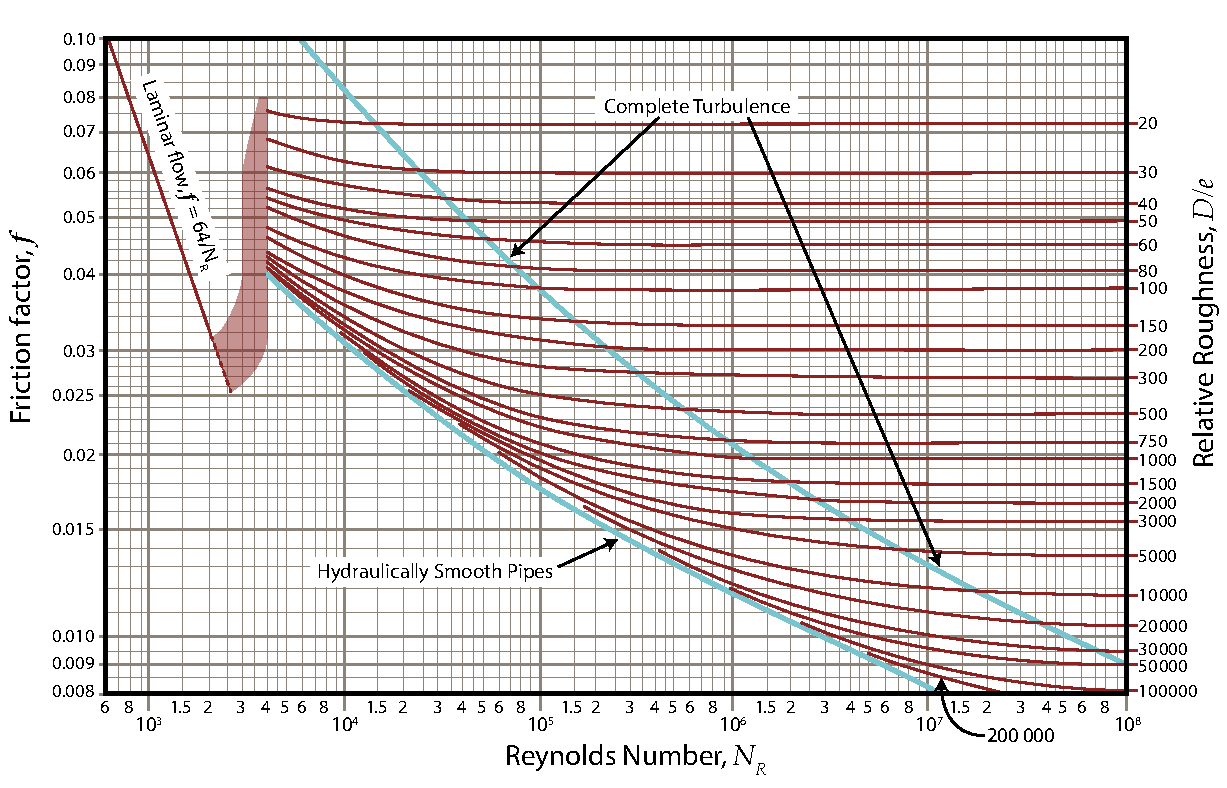
\includegraphics[angle=-90,scale=1.2]{../../Figs/07SeriesPipeline/moody}
	}
	
	
	
\end{document}
